\documentclass{article}
\usepackage[utf8]{inputenc}
\usepackage[spanish]{babel}
\usepackage{graphicx}
\usepackage{float}

\title{Práctica 3. Primera parte: Implementación de los ejemplos}
\author{Noelia Escalera Mejías \and Grupo DSD1}

\begin{document}
	\maketitle
	\section{Ejemplo 1}
	\begin{enumerate}
		\item Crear los archivos
		\begin{figure}[H]
			\centering
			
\includegraphics[totalheight=2cm]{img/1.png}
		\end{figure}
		\item Compilamos los {\it .java}.
		\begin{figure}[H]
			\centering
			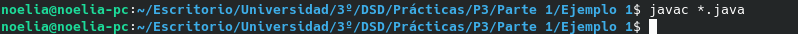
\includegraphics[totalheight=0.5cm]{img/2.png}
		\end{figure}
		\begin{figure}[H]
			\centering
			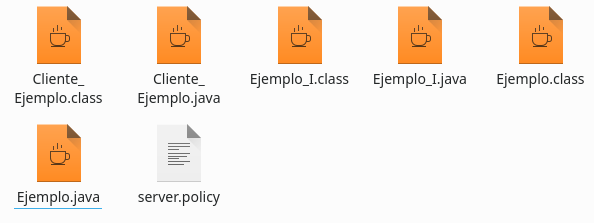
\includegraphics[totalheight=4cm]{img/3.png}
		\end{figure}
		\item Invocamos {\it rmiregistry}
		\begin{figure}[H]
			\centering
			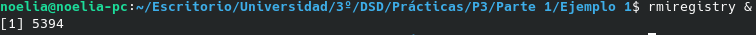
\includegraphics[totalheight=0.55cm]{img/4.png}
		\end{figure}
		\item Lanzamos el servidor
		\begin{figure}[H]
			\centering
			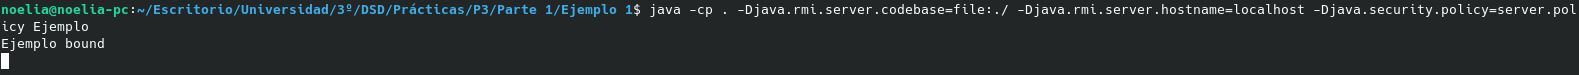
\includegraphics[totalheight=0.6cm]{img/5.png}
		\end{figure}
		\item Lanzamos el cliente
		\begin{figure}[H]
			\centering
			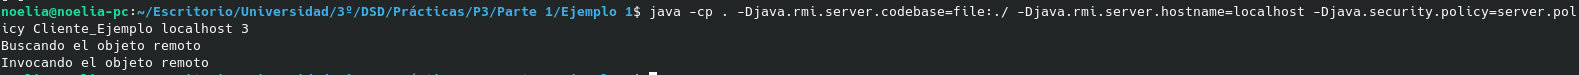
\includegraphics[totalheight=0.6cm]{img/6.png}
		\end{figure}
		En el servidor obtenemos esto:
		\begin{figure}[H]
			\centering
			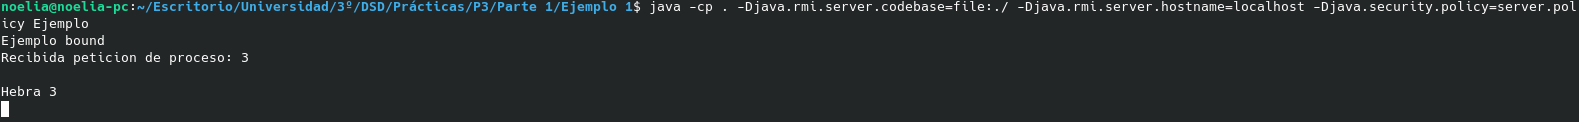
\includegraphics[totalheight=0.98cm]{img/7.png}
		\end{figure}
		Si le pasamos 0 como argumento al cliente:
		\begin{figure}[H]
			\centering
			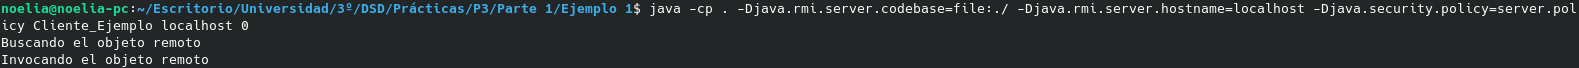
\includegraphics[totalheight=0.55cm]{img/8.png}
		\end{figure}
		\begin{figure}[H]
			\centering
			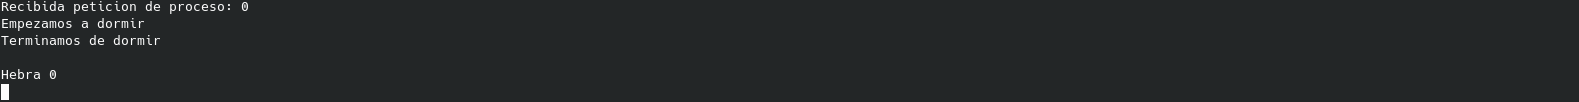
\includegraphics[totalheight=0.82cm]{img/9.png}
		\end{figure}
	\end{enumerate}
	Lo que está ocurriendo es que el cliente busca un objeto remoto, encuentra el que ha creado nuestro servidor y lo llama pasándole como argumento el que le hemos pasado nosotros. El servidor los interpreta como número de proceso y dependiendo de si es el proceso 0 o no hace un sleep o no.
	\section{Ejemplo 2}
	\begin{enumerate}
		\item Creamos los archivos
		\begin{figure}[H]
			\centering
			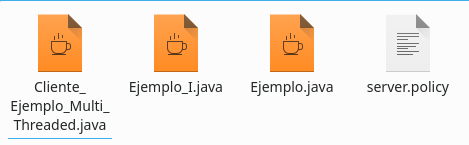
\includegraphics[totalheight=2cm]{img/10.png}
		\end{figure}
		\item Compilamos los {\it .java}.
		\begin{figure}[H]
			\centering
			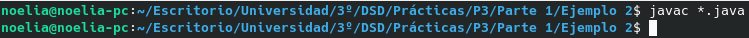
\includegraphics[totalheight=0.5cm]{img/11.png}
		\end{figure}
		\begin{figure}[H]
			\centering
			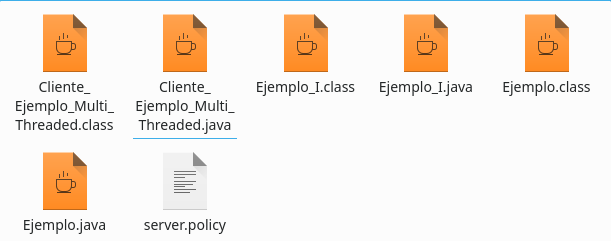
\includegraphics[totalheight=4cm]{img/12.png}
		\end{figure}
		\item Invocamos {\it rmiregistry}
		\begin{figure}[H]
			\centering
			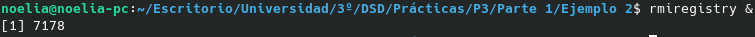
\includegraphics[totalheight=0.55cm]{img/13.png}
		\end{figure}
		\item Lanzamos el servidor
		\begin{figure}[H]
			\centering
			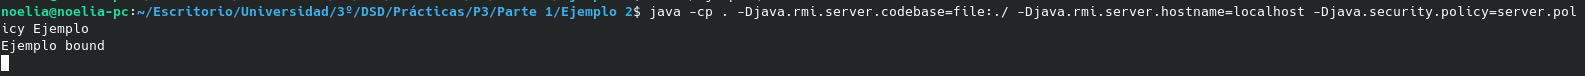
\includegraphics[totalheight=0.6cm]{img/14.png}
		\end{figure}
		\item Lanzamos el cliente
		\begin{figure}[H]
			\centering
			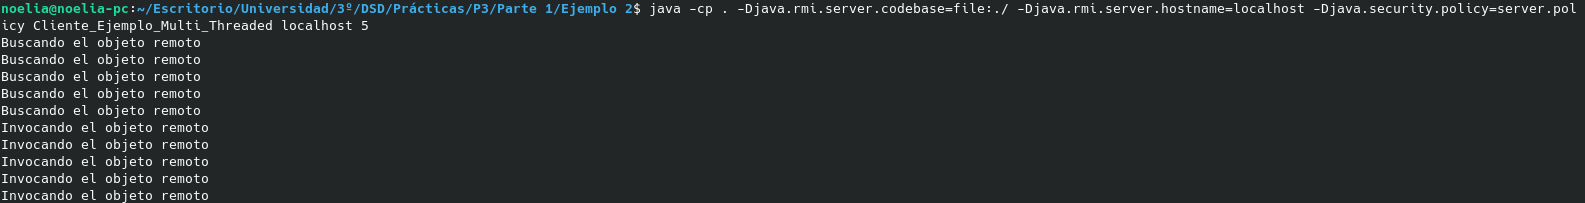
\includegraphics[totalheight=1.6cm]{img/15.png}
		\end{figure}
		En el servidor obtenemos esto:
		\begin{figure}[H]
			\centering
			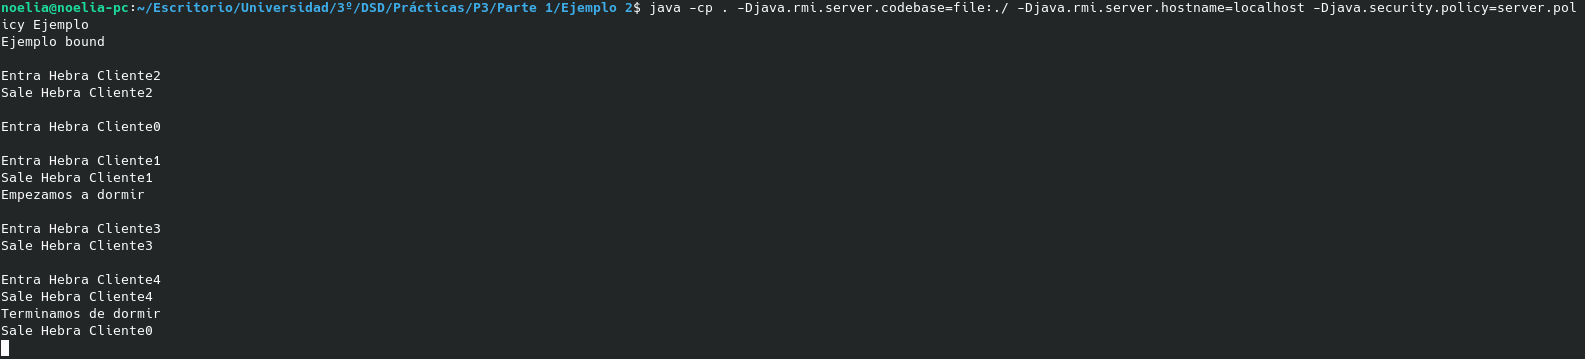
\includegraphics[totalheight=2.8cm]{img/16.png}
		\end{figure}
		
	\end{enumerate}
	Lo que ocurre aquí es que al cliente le pasamos como argumento el número de hebras que se quieren lanzar. El servidor hace sleep a los procesos múltiplos de 10.\\
	
	Si añadimos ahora el modificador synchronized:
	\begin{figure}[H]
		\centering
		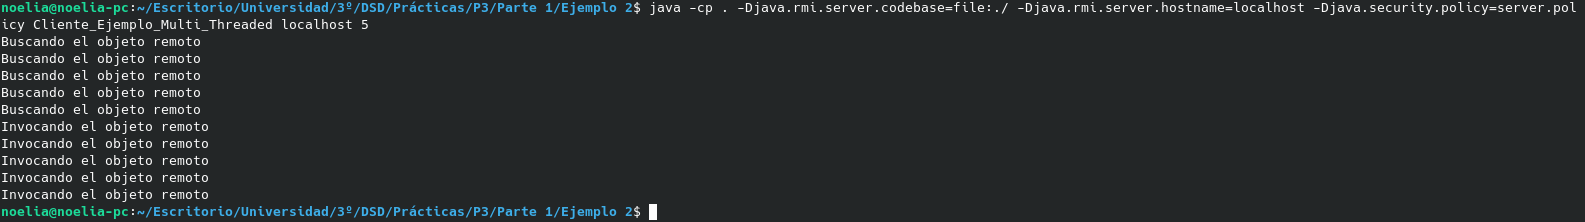
\includegraphics[totalheight=1.7cm]{img/17.png}
	\end{figure}
	\begin{figure}[H]
		\centering
		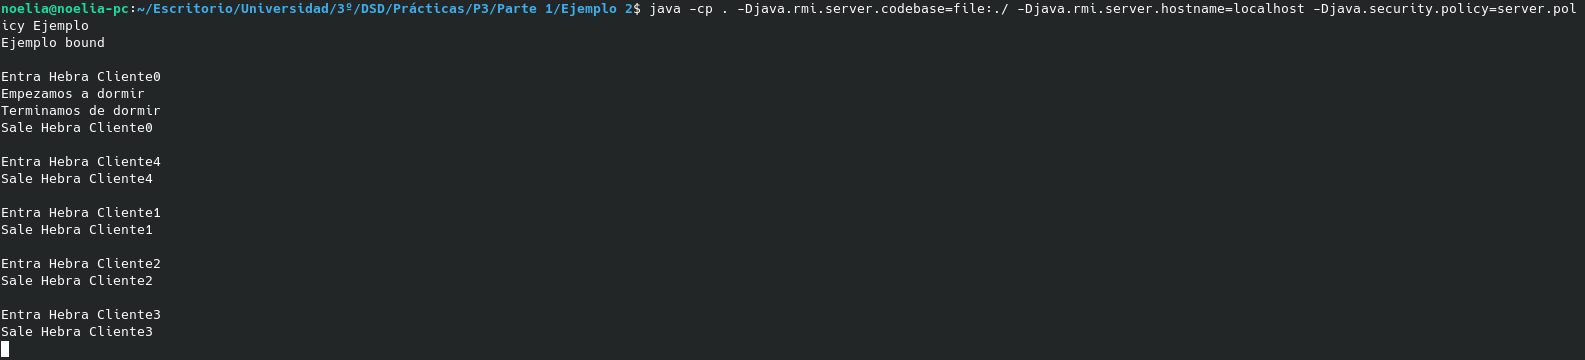
\includegraphics[totalheight=2.75cm]{img/18.png}
	\end{figure}
	Lo que ocurre ahora es que no se ejecuta una hebra hasta que se ha terminado de ejecutar la que estaba antes.
	
	\section{Ejemplo 3}
	\begin{enumerate}
		\item Creamos los archivos
		\begin{figure}[H]
			\centering
			
\includegraphics[totalheight=2cm]{img/19.png}
		\end{figure}
		\item Compilamos los {\it .java}.
		\begin{figure}[H]
			\centering
			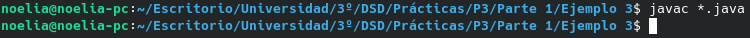
\includegraphics[totalheight=0.5cm]{img/20.png}
		\end{figure}
		\begin{figure}[H]
			\centering
			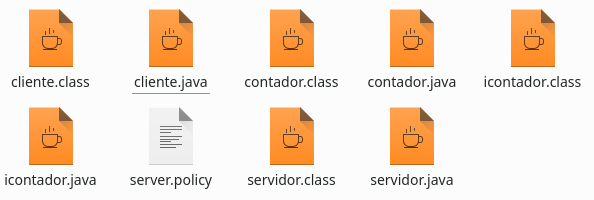
\includegraphics[totalheight=4cm]{img/21.png}
		\end{figure}
		\item Invocamos {\it rmiregistry}
		\begin{figure}[H]
			\centering
			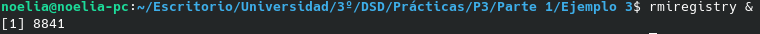
\includegraphics[totalheight=0.55cm]{img/22.png}
		\end{figure}
		\item Lanzamos el servidor
		\begin{figure}[H]
			\centering
			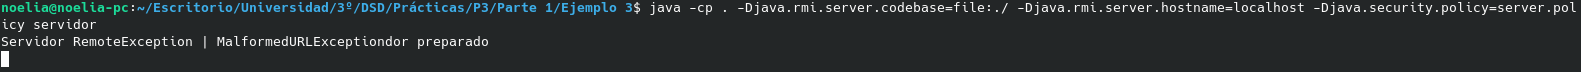
\includegraphics[totalheight=0.6cm]{img/23.png}
		\end{figure}
		Antes apareció el siguiente error:
		\begin{figure}[H]
			\centering
			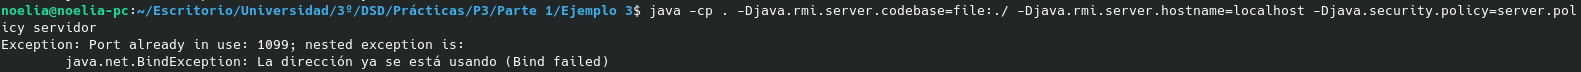
\includegraphics[totalheight=0.6cm]{img/24.png}
		\end{figure}
		Se ha solucionado cambiando el puerto en {\it servidor.java}
		\item Lanzamos el cliente
		\begin{figure}[H]
			\centering
			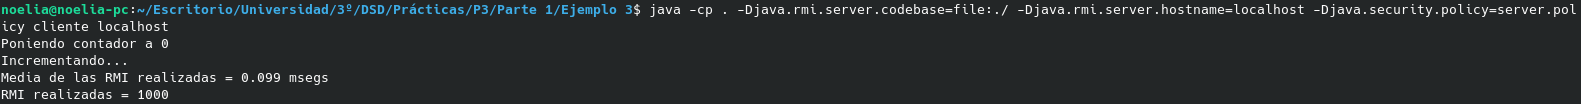
\includegraphics[totalheight=0.87cm]{img/25.png}
		\end{figure}
	\end{enumerate}
	Lo que ocurre aquí es que el servidor sirve un contador y el cliente lo llama 1000 veces.
\end{document}}